\documentclass[a4paper,12pt]{article}
\usepackage[spanish]{babel}
\usepackage[utf8]{inputenc}
\usepackage{booktabs}
\usepackage{dirtytalk}
\usepackage{graphicx}
\usepackage{makecell}
\usepackage[section]{placeins}

\begin{document}

\begin{titlepage}

\newcommand{\HRule}{\rule{\linewidth}{0.5mm}} % Defines a new command for the horizontal lines, change thickness here

\center % Center everything on the page
 
%----------------------------------------------------------------------------------------
%	HEADING SECTIONS
%----------------------------------------------------------------------------------------

\textsc{\LARGE Instituto Politécnico Nacional  Escuela Superior de Cómputo}\\[1.5cm] % Name of your university/college

\includegraphics[scale=.3]{escom.png}\\[1cm] % Include a department/university logo - this will require the graphicx package
\textsc{\Large Redes}\\[0.5cm] % Major heading such as course name
%\textsc{\large Course code}\\[0.5cm] % Minor heading such as course title

%----------------------------------------------------------------------------------------
%	TITLE SECTION
%----------------------------------------------------------------------------------------

\HRule \\[0.4cm]
{ \huge \bfseries Práctica 1 : Captura de tramas}\\[0.4cm] % Title of your document
\HRule \\[1.5cm]
 
%----------------------------------------------------------------------------------------
%	AUTHOR SECTION
%----------------------------------------------------------------------------------------

\begin{minipage}{0.6\textwidth}
\begin{flushleft} \large
%\emph{Author:}\\
\begin{center}
Integrantes:
\end{center}
\begin{itemize}
\item Hernández Escobedo Fernando
\item Meza Zamora  Abraham Manuel 
\end{itemize}
\end{flushleft}

\end{minipage}\\[2cm]

% If you don't want a supervisor, uncomment the two lines below and remove the section above
%\Large \emph{Author:}\\
%John \textsc{Smith}\\[3cm] % Your name

%----------------------------------------------------------------------------------------
%	DATE SECTION
%----------------------------------------------------------------------------------------

{\large \today}\\[2cm] % Date, change the \today to a set date if you want to be precise

\vfill % Fill the rest of the page with whitespace

\end{titlepage}

\section{Introducción}
En informática, un \textit{Sniffer} es un programa de captura de las tramas de una red de computadoras.

Es algo común que, por topología de red y necesidad material, el medio de transmisión (cable coaxial, cable de par trenzado, fibra óptica, etc.) sea compartido por varias computadoras y dispositivos de red, lo que hace posible que un ordenador capture las tramas de información no destinadas a él. Para conseguir esto el analizador pone la tarjeta de red en un estado conocido como "modo promiscuo" en el cual en la capa de enlace de datos no son descartadas las tramas no destinadas a la dirección MAC de la tarjeta; de esta manera se puede capturar (sniff, "olfatear") todo el tráfico que viaja por la red.
.
\section{Desarrollo}
\begin{itemize}
\item En C
\begin{enumerate}
\item Simplemente, leímos el pdf, y seguimos las instrucciones paso a paso para llevar a cabo la instalación.
\item Compilamos el programa y observamos la salida (fig1) y (fig2).
\end{enumerate}
\item En Java
\begin{enumerate}
\item Seguimos las instrucciones de instalación del pdf.
\item Observé la salida. A diferencia del ejemplo en C, mostraba la trama sin formato.
\item Basado en el ejemplo de encabezados vistos en clase, hicimos una modificación al código de captura, iterando un ciclo \texttt{for} sobre la trama. Inicializando \texttt{i} de manera adecuada para mostrar de manera adecuada:
\begin{enumerate}
\item MAC destino
\item MAC destino
\item MAC tipo
\end{enumerate}
\item Finalmente compilamos el código y observamos las tramas capturadas. (fig3).
\end{enumerate} 
\end{itemize}
\section{Pruebas}
\begin{figure}[h]
\center
\includegraphics[scale=.5]{fig1}
\caption{Captura de tramas en C}
\end{figure}
\begin{figure}[h]
\center
\includegraphics[scale=.5]{fig2}
\caption{Formato de captura de tramas}
\end{figure}

\begin{figure}[h]
\center
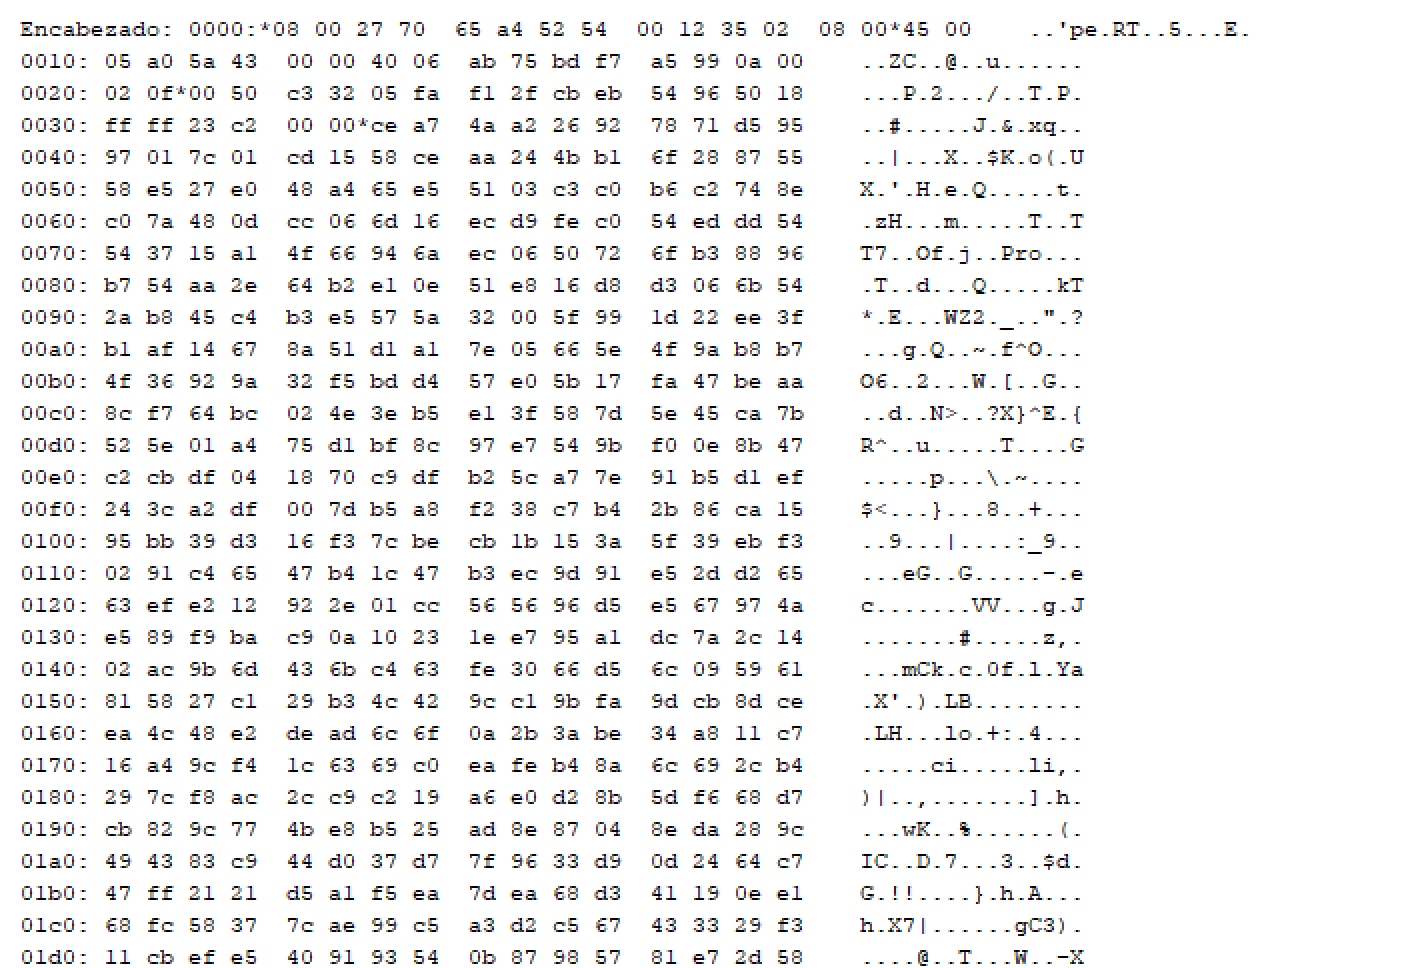
\includegraphics[scale=.5]{fig3}
\caption{Captura de tramas en Java, encabezado sin formato}
\end{figure}

\begin{figure}[h]
\center
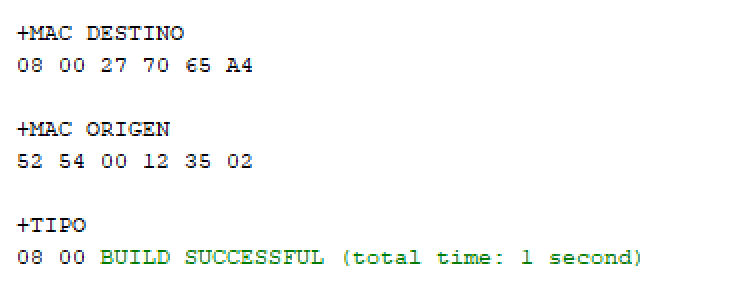
\includegraphics[scale=.5]{fig4}
\caption{Trama con formato adecuado}
\end{figure}

\section{Conclusiones}
\begin{itemize}
\item Fernando: Este tipo de aplicaciones tienen la responsabilidad de realizar la captura de distintos paquetes que se encuentran en circulación a través de una red informática.  Además de esto, los sniffers tienen un uso fundamental, que viene a ser el de analizar los paquetes de la red y estudiarlos, no solo capturarlos.

\item Abraham :La práctica realizada tuvo como objetivo sentar las bases para poder interpretar los mensajes que utilizan los dispositivos para comunicarse,además  analizadores de paquetes tienen diversos usos, como monitorear redes para detectar y analizar fallos, o para realizar ingeniería inversa en protocolos de red. También es habitual su uso para fines maliciosos, como robar contraseñas, interceptar correos electrónicos, espiar conversaciones de chat, etc.
\end{itemize}
\end{document}